\documentclass{article}

\usepackage[T1]{fontenc}    %Schriftart des Dokumentes
\usepackage[ngerman]{babel} %Dokumentensprache, hier Deutsch
\usepackage{amsmath, amssymb, stmaryrd} %mathematische Schriftzeichen
\usepackage{graphicx} %Einfügen von Grafiken
\usepackage{wrapfig}
\usepackage{bm}
\usepackage{subfig}
\usepackage{newclude}
\usepackage{pdfpages}

\setlength{\parindent}{0pt} %Einrückung von Absätzen auf null gesetzt
\setlength{\parskip}{10pt} %Abstand zischen Absätzen auf 10pt gesetzt

\title{Versuch 221: Adiabatenkoeffizient}
\author{Matthias Kuntz}
\date{29.02.2024}

\renewcommand*\contentsname{Zusammenfassung}

\begin{document}

\maketitle

\tableofcontents

\newpage

%-------------------------EINLEITUNG-------------------------
\section{Einleitung}

Thermische Prozesse bilden einen der Grundbausteine der physikalischen Welt. Eine bestimmte Art von diesen sind die Adiabatischen Prozesse, welche die Gleichung $pV^\kappa = \text{konst.}$ erfüllen. Und um genau dieses $\kappa$, den sogenannten Adiabatenkoeffizienten, geht es in diesem Versuch. Diese temperaturabhängige Materialeigenschaft soll mit zwei verschiedenen Methoden bestimmt werden, einmal mit einem Aufbau nach Clément-Desormes und einmal mit einem Versuch nach Rüchard. Dabei bestimmen wir bei Ersterem Druckunterschiede an verschieden Stellen eines thermischen Prozesses und bei Letzterem die Periodendauer einer durch adiabatische Kompression angeregten Schwingung.  

\subsection{Physikalische Grundlagen}

\subsubsection{Messung des Adiabatenkoeffizienten nach Clément und Desormes}

\begin{figure}[h]
  \centering
  \subfloat[Versuchsaufbau]{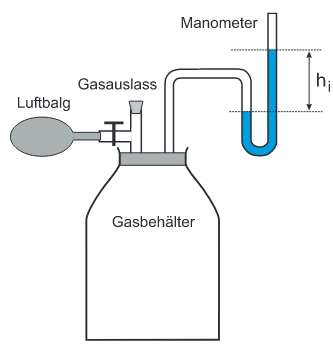
\includegraphics[width=0.4\textwidth]{graphics/CD-Aufbau.png}\label{fig:CD-Aufbau}}
  \hfill
  \subfloat[pV-Diagramm]{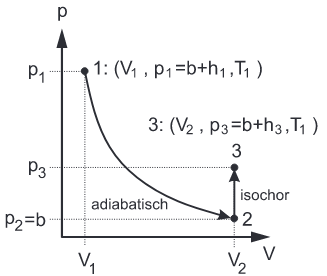
\includegraphics[width=0.48\textwidth]{graphics/CD-PV.png}\label{fig:CD_PV}}
  \hfill
  \caption{Versuch nach Clément-Desormes [Quelle: PAP2.1 Skript, S.29, 03.03.2024]}
  \label{fig:CD}
\end{figure}

In Abbildung \ref{fig:CD} ist der Aufbau des Versuchs sowie das zugehörige pV-Diagramm dargestellt. Man beginnt, indem man mit dem Luftbalg Luft in den Gasbehälter pumpt und somit einen Überdruck erzeugt. Dabei erwärmt sich das Gas und erreicht somit nach kurzem Abkühlen auf Raumtemperatur den Zustand 1 im pV-Diagramm, welcher beschrieben wird durch:

\begin{equation}
    \textbf{Zustand 1:} \ \ \ V_1, \ \ \ p_1 = b + h_1, \ \ \ T_1.
\end{equation}

Dabei bezeichnen $V_1$ das Volumen des Gasbehälters, $b$ den äußeren Luftdruck, $h_1$ die hier abzulesende Höhendifferenz des Manometers und $T_1$ die Temperatur des Gases, ergo in diesem Fall die Raumtemperatur.

Nun wird für eine kurze Zeit der Gasauslass geöffnet. Dies kann beschrieben werden durch einen adiabatischen Prozess, bei dem sich das Gas ohne Wärmeaustausch dem äußeren Luftdruck $b$ anpasst. Das entwichene Gas kann genauso gut beschreiben werden als eine Expansion des Volumens um $\Delta V$, bis der Druck $b$ erreicht ist. Die Temperatur nimmt hierbei auch um den Wert $\Delta T$ ab, wodurch Zustand 2 im pV-Diagramm erreicht wird und sich folgende zusammenfassende Beschreibung ergibt:

\begin{equation}
    \textbf{Zustand 2:} \ \ \ V_2 = V_1 + \Delta V, \ \ \ p_2 = b, \ \ \ T_2 = T_1 - \Delta T.
\end{equation}

Zuletzt wartet man erneut ab, bis sich die Temperatur wieder der Raumtemperatur angeglichen hat. Dies entspricht einem isochoren Prozess, bei dem der Druck ansteigt und Zustand 3 erreicht wird:

\begin{equation}
    \textbf{Zustand 3:} \ \ \ V_3 = V_2 = V_1 + \Delta V, \ \ \ p_3 = b + h_3, \ \ \ T_3 = T_1.
\end{equation}

Nun da wir den thermischen Prozess komplett beschrieben haben können wir herleiten, wie man allein durch die Messungen von $h_1$ und $h_3$ den Adiabatenkoeffizienten bestimmen kann.

Wir beginnen, indem wir die Zustände 1 \& 2 über die Poisson'sche Gleichung für adiabatische Prozesse verbinden und die jeweiligen Formen der Zustände einsetzen:

\begin{equation}
    \begin{split}
        p_1 V_1^\kappa &= p_2 V_2^\kappa \\
        (b + h_1) V_1^\kappa &= b (V_1 + \Delta V)^\kappa
    \end{split}
\end{equation}

Wir können, da $\Delta V \ll V_1$ ist, den Term für $V_2$ folgendermaßen nähern:

\begin{equation}
    (V_1 + \Delta V)^\kappa = V_1^\kappa \left( 1 + \frac{\Delta V}{V_1} \right)^\kappa \approx V_1^\kappa \left( 1 + \kappa \frac{\Delta V}{V_1} \right).
\end{equation}

Setzen wir dies oben ein so erhalten wir die Folgende Form für den Übergang von 1 zu 2:

\begin{equation}
    \frac{h_1}{b} = \kappa \frac{\Delta V}{V_1}.
    \label{eq:12}
\end{equation}

Für die Zustände 1 \& 3 haben wir jeweils die gleiche Temperatur, somit gilt durch das Boyle-Mariotte'sche Gesetz:

\begin{equation}
    \begin{split}
        p_1 V_1 &= p_3 V_3 \\
        (b + h_1) V_1 &= (b + h_3) (V_1 + \Delta V).
    \end{split}
\end{equation}

Auf der rechten Seite dieser Gleichung kann beim ausmultiplizieren der Term $h_3 \cdot \Delta V$ vernachlässigt werden, da jeweils $h_3 \ll b$ und $\Delta V \ll V_1$ gilt. Somit ergibt sich für diese Gleichung die Form:

\begin{equation}
    \begin{split}
        h_1 V_1 &= h_3 V_1 + b \cdot \Delta V \\
        \frac{\Delta V}{V_1} &= \frac{h_1 - h_3}{b}.
    \end{split}
\end{equation}

Setzen wir diesen Ausdruck in Gleichung \ref{eq:12} ein so erhält man folgende Formel für den Adiabatenkoeffizienten:

\begin{equation}
    \kappa = \frac{h_1}{h_1 - h_3}.
    \label{eq:CD_kappa}
\end{equation}

\subsubsection{Messung des Adiabatenkoeffizienten nach Rüchard}

\begin{figure}
    \centering
    \includegraphics[width=0.48\textwidth]{graphics/Rü-Aufbau.png}
    \caption{Versuchsaufbau nach Rüchard [Quelle: PAP2.1 Skript, S.30, 03.03.2024]}
    \label{fig:Rü-Aufbau}
\end{figure}

Der Aufbau diese Versuchsteils ist in Abbildung \ref{fig:Rü-Aufbau} zu sehen. Hierbei befindet sich ein Glasrohr auf einem Gasbehälter, in dem ein Schwingkörper eingelassen ist, welcher nahezu den gleichen Radius wie das Rohr besitzt. Wird nun über die Gasflasche der Gasbehälter kontinuierlich mit Gas befüllt, so beginnt der Schwingkörper im Rohr auf und ab zu schwingen. Dabei oszilliert er um eine kleine Öffnung im Rohr, durch die das zugeführte Gas immer entfliehen kann. So entsteht eine Schwingung des Körpers basierend auf der adiabatischen Kompression des Gases. Der Druck im Gasbehälter setzt sich währenddessen zusammen aus dem Luftdruck $p_0$ sowie dem Schweredruck des Schwingkörpers:

\begin{equation}
    p = p_0 + \frac{mg}{A} = p + \frac{mg}{\pi r^2}.
    \label{eq:Druck}
\end{equation}

Hierbei stehen $m$ und $r$ für die Masse beziehungsweise den Radius des Körpers und $g$ steht wie gewohnt für die Gravitationsbeschleunigung. $A = \pi r^2$ bezeichnet somit die Querschnittsfläche des Schwingkörpers im Rohr.

Man kann nun nach Newton die Bewegungsgleichung für den Schwingkörper aufstellen. Bewegt sich dieser um eine kleine Strecke $x$ über die Gleichgewichtslage hinaus, so ändert sich der Druck $p$ um einen Wert d$p$ und es gilt:

\begin{equation}
    m \ddot{x} = A \ \text{d}p
    \label{eq:Newton}
\end{equation}

Allgemein passiert der Vorgang adiabatisch, wodurch erneut $pV^\kappa = \text{konst.}$ gilt. Differenziert man diesen Ausdruck nach V so erhält man:

\begin{equation}
    \begin{split}
        p &= V^{-\kappa} \cdot \text{konst.} \\
        \frac{dp}{dV} &= - \kappa V^{-\kappa -1} \cdot \text{konst.} \\
        \frac{dp}{dV} &= - \kappa \frac{p}{V} \\
        dp &= - \kappa \frac{p}{V} dV
    \end{split}
\end{equation}

Diesen Ausdruck kann man nun in Gleichung \ref{eq:Newton} einsetzen. Verwendet man zusätzlich die Beziehung d$V = Ax = \pi r^2 x$ mit dem Rohrradius $r$ so erhält man:

\begin{equation}
    \begin{split}
        m \ddot{x} = - \kappa \frac{p}{V} A^2 x &= - \pi^2 r^4 \kappa \frac{p}{V} x \\
        \iff \ \ \ddot{x} + \frac{\pi^2 r^4 \kappa p}{mV} x &= 0.
    \end{split}
    \label{eq:Bew_Rü}
\end{equation}

Dies entspricht genau der Form eines harmonischen Oszillators $\ddot{x} + \omega^2 x = 0$, für welchen wir die Lösung kennen: Eine harmonische Schwingung mit der Kreisfrequenz $\omega$ und der Periodendauer $T = 2 \pi / \omega$. Vergleichen wir also diese Form mit Gleichung \ref{eq:Bew_Rü}, so erhalten wir:

\begin{equation}
    T = \sqrt{\frac{4mV}{r^4 \kappa p}}.
\end{equation}

Somit kommen wir zu dem Ergebnis, dass man mit der Messung der Periodendauer $T$ den Adiabatenkoeffizienten bestimmen kann:

\begin{equation}
    \kappa = \frac{4mV}{r^4 T^2 p}.
    \label{eq:Rü_Kappa}
\end{equation}

Dabei bezeichnen die Größen $m$, $V$ und $r$ die Parameter des Versuchsaufbaus und $p$ den über Gleichung \ref{eq:Druck} bestimmten Druck. 

%---------------VERSUCHSPROTOKOLL MIT MESSDATEN---------------
\newpage

\section{Versuchsprotokoll mit Messdaten}

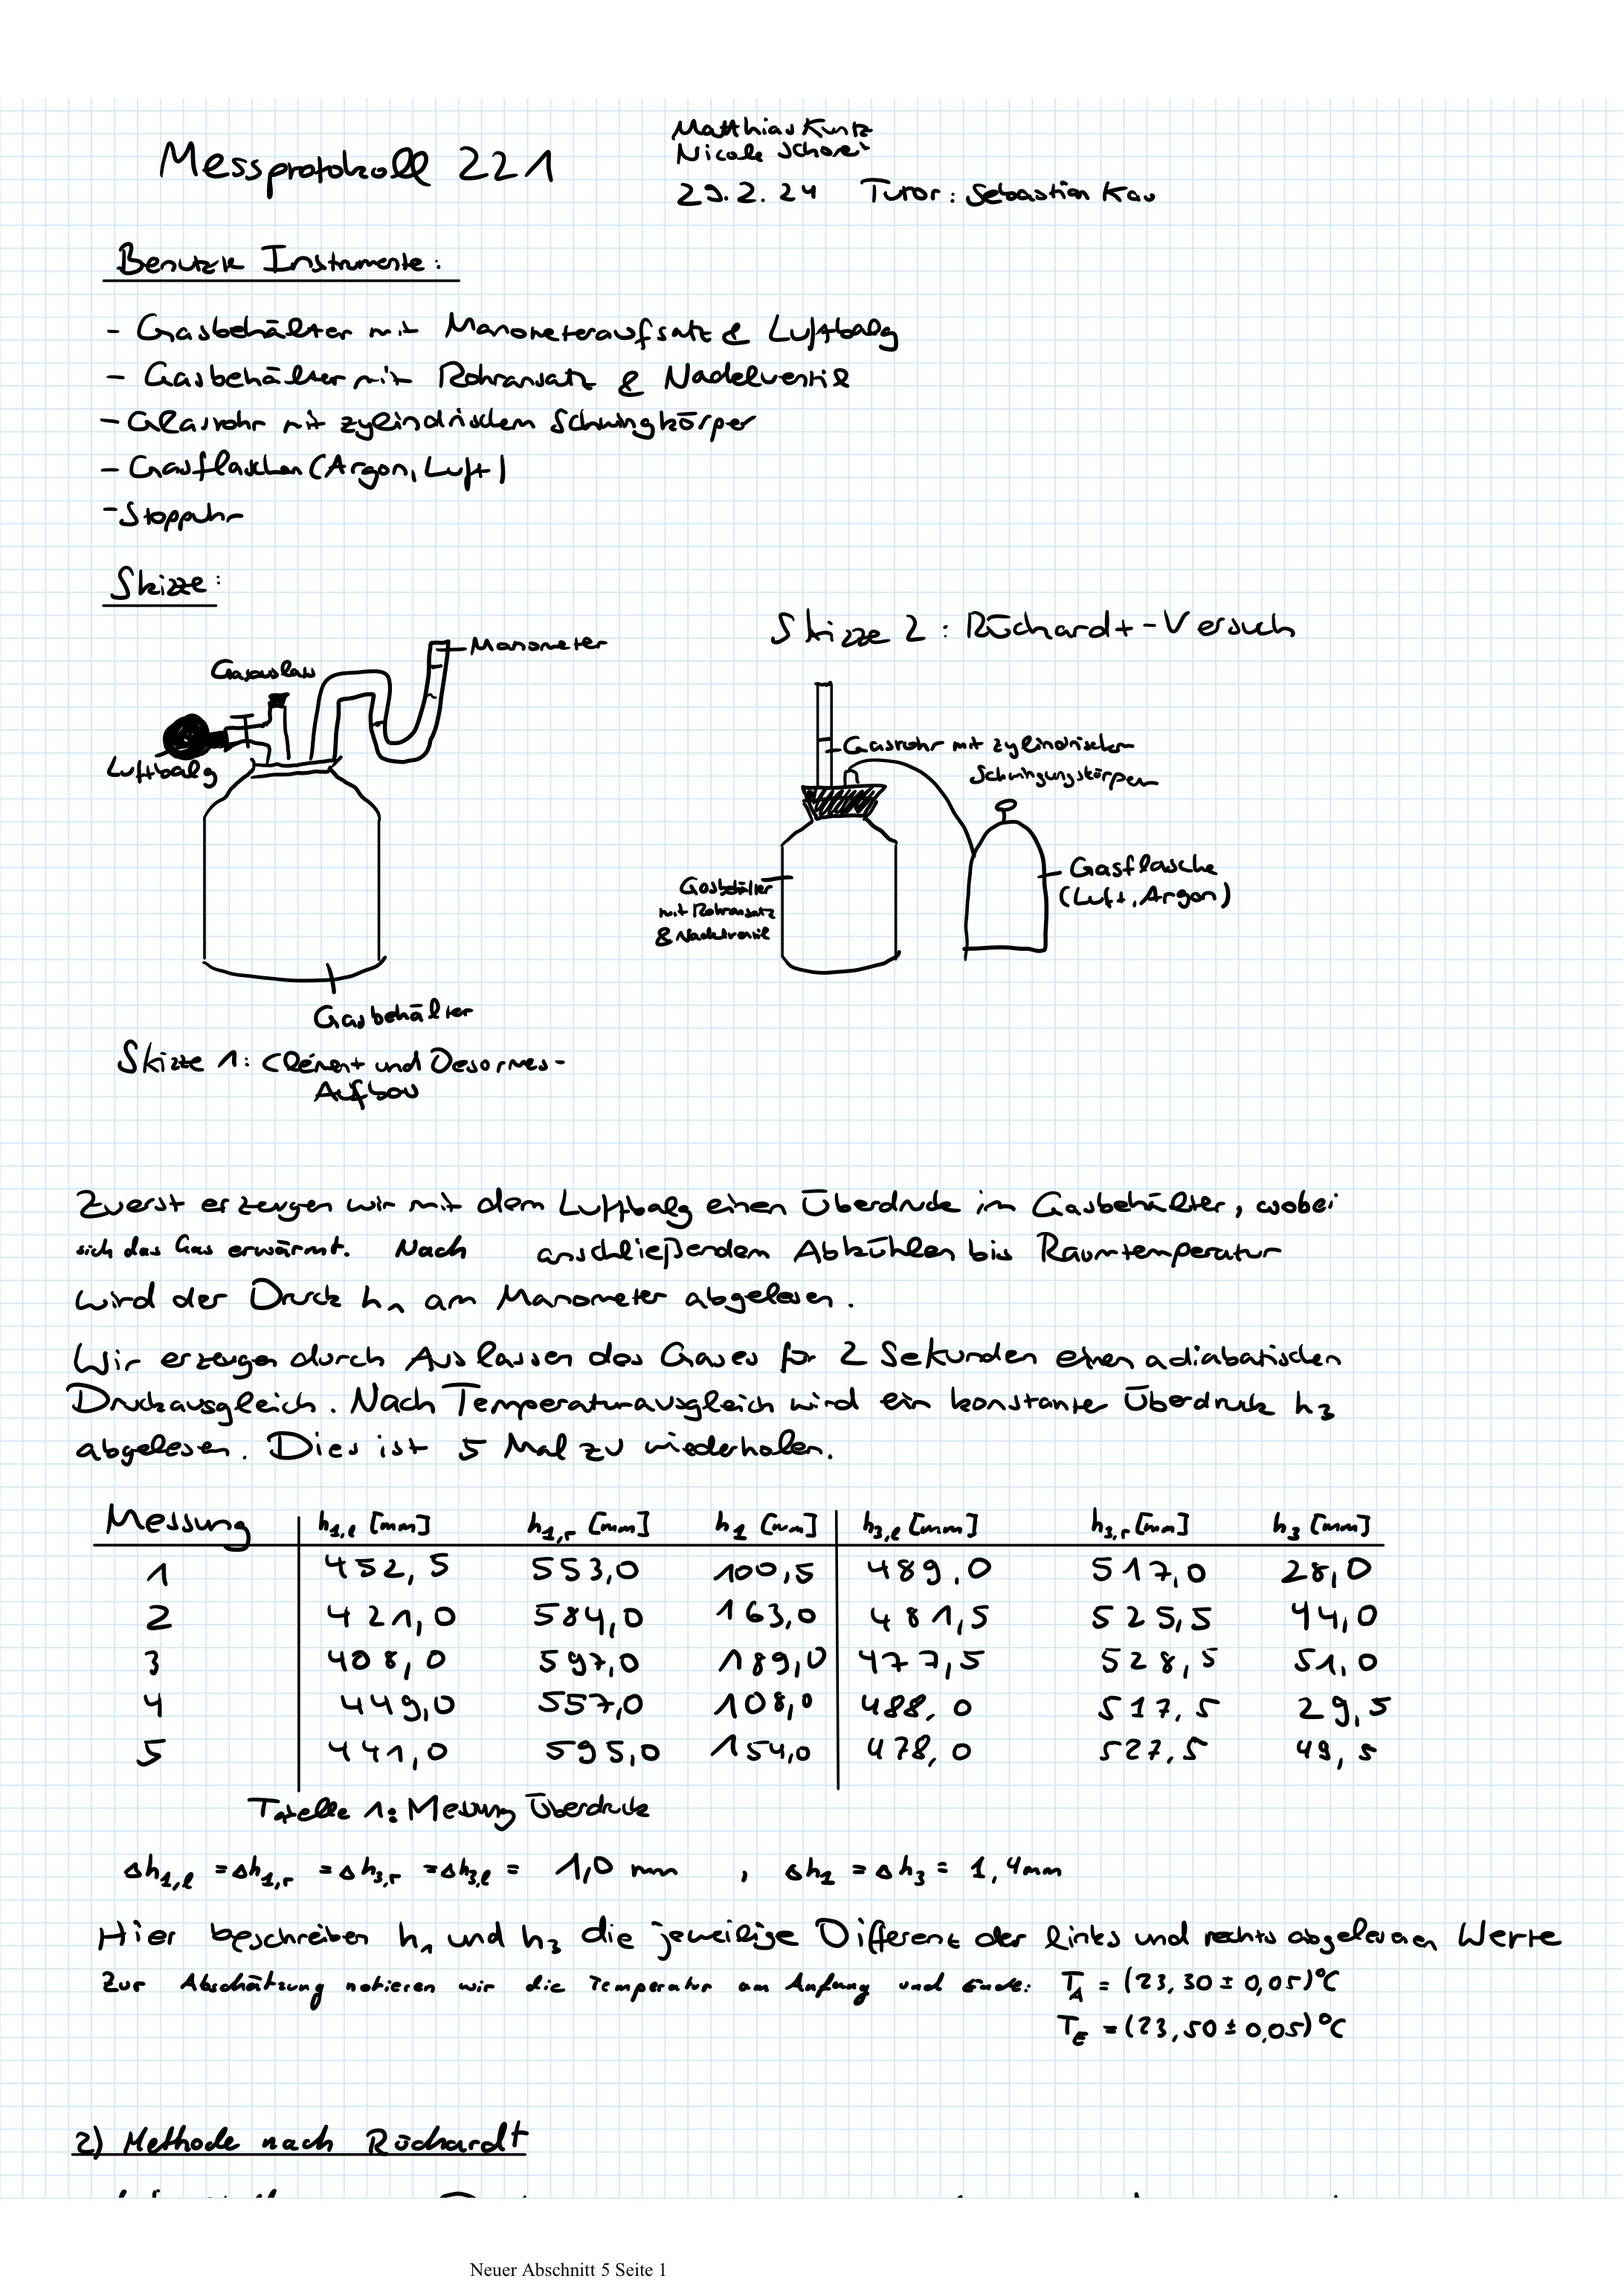
\includegraphics[width=\textwidth]{graphics/mess1.jpg}
\newpage
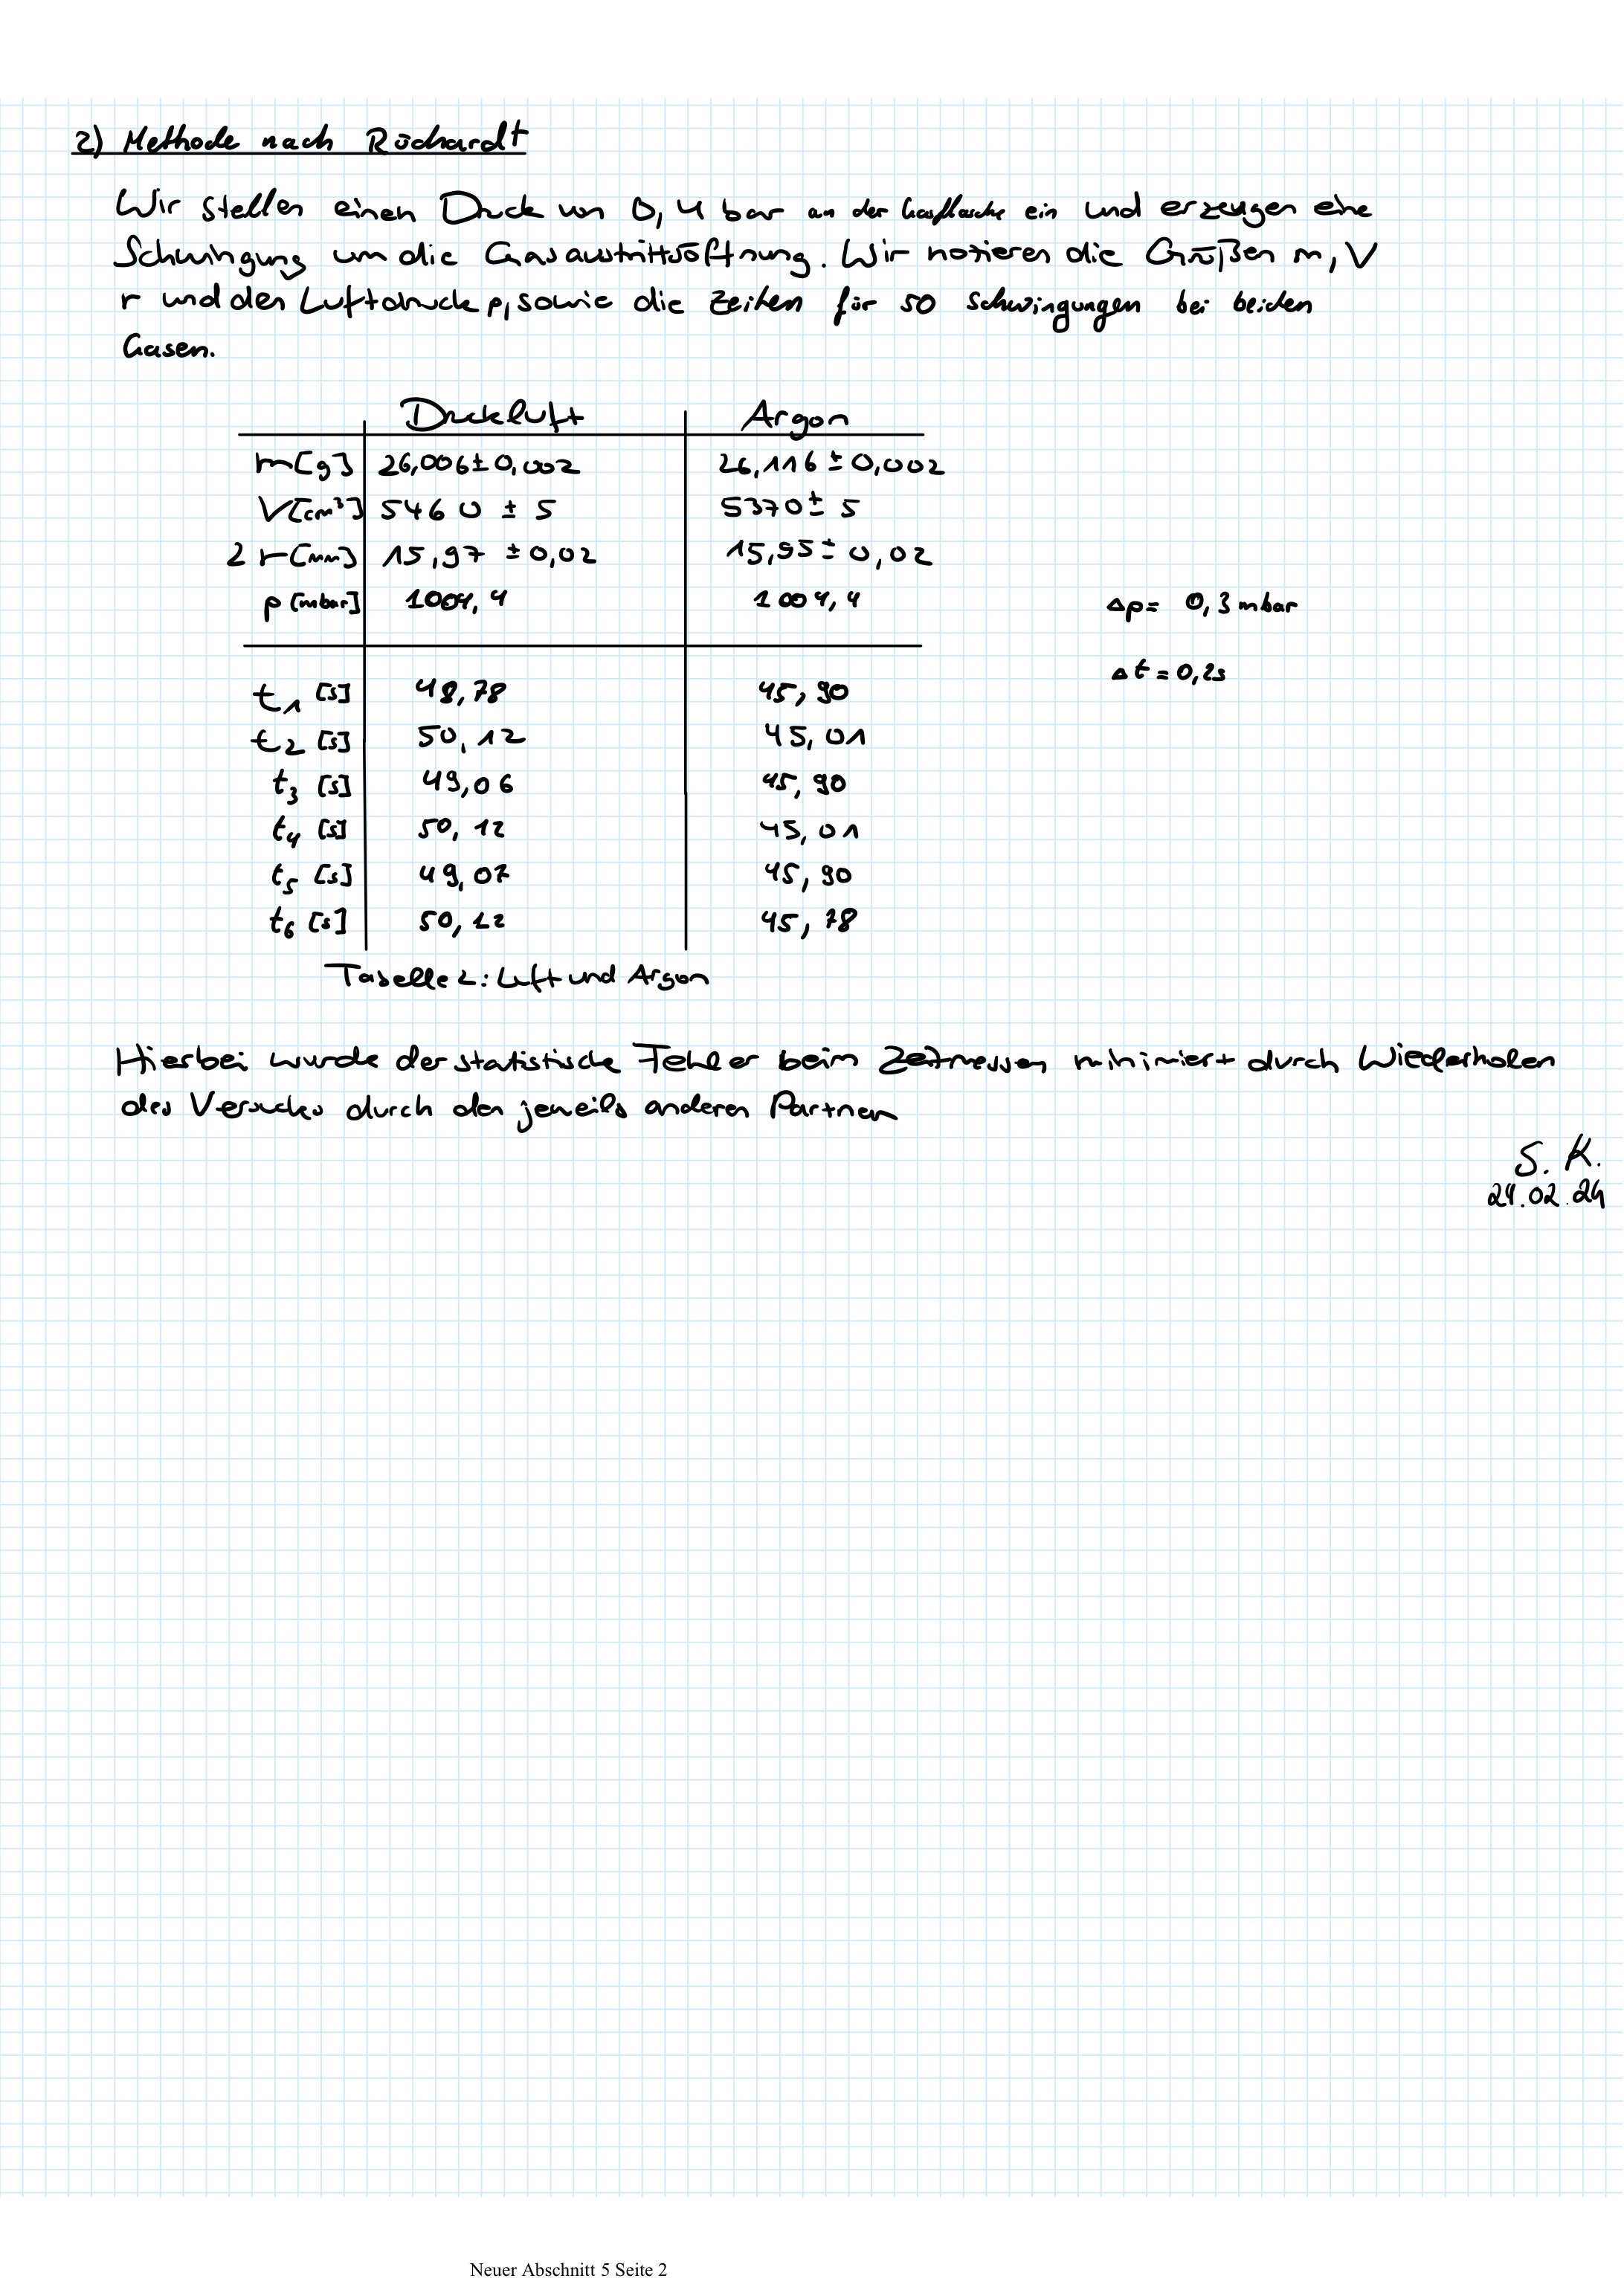
\includegraphics[width=\textwidth]{graphics/mess2.jpg}
\newpage

\addtocounter{table}{2}

\newpage
%-------------------------AUSWERTUNG-------------------------
\section{Auswertung}

In dieser Evaluation werden alle Fehler, sofern keine spezifische Angabe gemacht wird, mithilfe der Gauss'schen Fehlerfortpflanzung berechnet. Dies bedeutet, dass ein Wert $F$, der mit der Formel $f(a_1, ..., a_n)$ berechnet wird, den Fehler $\Delta F$ annimmt:

\begin{equation}
    \Delta F = \sqrt{\sum_n \left( \frac{\partial f}{\partial a_n} \cdot \Delta a_n \right)^2}.
\end{equation}

Des Weiteren erfolgen Signifikanztests von zwei Werten $a$ und $a'$ über die folgende Formel:

\begin{equation}
    \sigma = \frac{|a-a'|}{\sqrt{(\Delta a)^2 + (\Delta a')^2}}.
\end{equation}

Die Güte eines Fits wird mit der $\chi^2$-Summe bewertet:

\begin{equation}
    \chi^2 = \sum_i^N \left( \frac{\textit{Funktionswert}_i - \textit{Messwert}_i}{\textit{Fehler}_i} \right)^2
\end{equation}

Auch verwendet wird $\chi^2_{red} = \chi^2 / f$, wobei der Freiheitsgrad $f$ die Anzahl der Messwerte minus die Anzahl der Fitparameter ist. Der auf die Freiheitsgrade normierte Wert soll bei einem guten Fit ungefähr 1 sein.

\newpage

\subsection{Bestimmung des Adiabatenkoeffizienten nach Clément-Desormes}

Wir beginnen mit der Auswertung der Manometer-Höhenwerte aus Tabelle 1 des Messprotokolls. Wir berechnen nach Gleichung \ref{eq:CD_kappa} für alle fünf Messungen den Adiabatenkoeffizient $\kappa_{CD}$. Der Fehler lässt sich dabei folgendermaßen berechnen:

\begin{equation}
    \Delta \kappa_{CD} = \frac{1}{(h_1 - h_3)^2} \sqrt{(h_3 \cdot \Delta h_1)^2 + (h_1 \cdot \Delta h_3)^2}.
\end{equation}

Wir tragen die Ergebnisse in Tabelle \ref{tab:kappa_CD} ein.

\phantom{.}

\begin{table}[!h]
    \centering
    %\resizebox{\textwidth}{!}{
    \begin{tabular}{cccc}
        \hline
        \textbf{Messung} & $\bm{h_1}$ [mm] & $\bm{h_3}$ [mm] & $\bm{\kappa_{CD}}$  \\ \hline
        1 & $100,5 \pm 1,4$ & $28,0 \pm 1,4$ & $1,386 \pm 0,028$     \\
        2 & $163,0 \pm 1,4$ & $44,0 \pm 1,4$ & $1,370 \pm 0,017$     \\
        3 & $189,0 \pm 1,4$ & $51,0 \pm 1,4$ & $1,370 \pm 0,014$     \\
        4 & $108,0 \pm 1,4$ & $29,5 \pm 1,4$ & $1,376 \pm 0,025$     \\
        5 & $154,0 \pm 1,4$ & $49,5 \pm 1,4$ & $1,474 \pm 0,021$     \\ \hline
    \end{tabular}%}
    \caption{Adiabatenkoeffizient für jede Messung}
    \label{tab:kappa_CD}
\end{table}

\phantom{.}

Aus den so berechneten Werten für Kappa bestimmen wir den Mittelwert und somit unser erstes Ergebnis für den Adiabatenkoeffizienten von Luft $\kappa_{L1}$. Der Fehler berechnet sich aus dem Standardfehler des Mittelwerts $\sigma_{MW}$ sowie den Messfehlern $\Delta \kappa_{CD}$:

\begin{equation}
    \Delta \kappa_{L1} = \sqrt{\sigma_{MW}^2 + (\Delta \kappa_{CD})^2}.
\end{equation}

Somit erhalten wir den Wert:

\begin{equation}
    \kappa_{L1} = 1,395 \pm 0,028
\end{equation}

Wir vergleichen diesen Wert über einen Signifikanztest mit dem Literaturwert für Stickstoff $\kappa_{N2} = 1,401$ und erhalten eine Abweichung von $\sigma_{L1} = 0,21$, was gut im $1\sigma$-Bereich liegt und somit nicht signifikant ist. 

\subsection{Bestimmung des Adiabatenkoeffizienten nach Rüchard}

Für die Bestimmung des Adiabatenkoeffizienten nach Rüchard verwenden wir Gleichung \ref{eq:Rü_Kappa} und bestimmen dazu zunächst aus den von uns gemessenen Zeiten aus Tabelle 2 des Messprotokolls die Zeit für eine Schwingung, indem wir die Messwerte durch die Anzahl gemessener Schwingungen, in diesem Fall bei allen 50, teilen. Der Fehler wird wie gewohnt nach Gauß auch durch eine Division mit 50 aus dem Messfehler $\Delta t$ bestimmt. Nun bestimmen wir den Mittelwert der Periodendauern. Erneut setzt sich der Fehler der Mittelwerte zusammen aus den Standartfehlern $\sigma_{MW}$ sowie den angegebenen Messfehlern $\Delta t$:

\begin{equation}
    \Delta T = \sqrt{\sigma_{MW}^2 + \left( \frac{\Delta t}{50} \right)^2}.
\end{equation}

Wir erhalten also die Werte für die Periodendauer einer Schwingung einmal für Luft und einmal für Argon:

\begin{equation}
    \begin{split}
        T_L &= (0,991 \pm 0,006) \text{s} \\
        T_{Ar} &= (0,912 \pm 0,005) \text{s}
    \end{split}
\end{equation}

Auch berechnen wir noch den jeweiligen Druck nach Gleichung \ref{eq:Druck} unter Verwendung der in Tabelle 2 gegeben Werte für den Luftdruck $p_0$, die Masse $m$ sowie den Radius $r$. Die Fehler berechnen sich somit nach:

\begin{equation}
    \Delta p = \sqrt{\left( \Delta p_0 \right)^2 + \left( \frac{g}{\pi r^2} \cdot \Delta m \right)^2 + \left( \frac{2mg}{\pi r^3} \cdot \Delta r \right)^2}.
\end{equation} 

Wir erhalten also die beiden Werte:

\begin{equation}
    \begin{split}
        p_L &= (101,71 \pm 0,03) \cdot 10^3 \ \text{Pa} \\
        p_{Ar} &= (101,72 \pm 0,03) \cdot 10^3 \ \text{Pa}
    \end{split}
\end{equation}

Damit können wir nun nach Gleichung \ref{eq:Rü_Kappa} die Adiabatenkoeffizienten bestimmen. Wir verwenden die im Messprotokoll jeweils in Tabelle 2 notierten Werte für $m$, $V$ und $r$ und bestimmen den Fehler für beide Fälle nach der Form:

\begin{equation}
    \Delta \kappa = \kappa \sqrt{\left( \frac{\Delta m}{m} \right)^2 + \left( \frac{\Delta V}{V} \right)^2 + \left( 4 \frac{\Delta r}{r} \right)^2 + \left( 2 \frac{\Delta T}{T} \right)^2 + \left( \frac{\Delta p}{p} \right)^2}.
\end{equation}

Somit erhalten wir:

\begin{equation}
    \begin{split}
        \kappa_{L2} &= 1,399 \pm 0,019 \\
        \kappa_{Ar} &= 1,640 \pm 0,021
    \end{split}
\end{equation}

Wir vergleichen die Werte erneut über Signifikanztests mit Literaturwerten. Für Luft verwenden wir wieder den von Stickstoff und für Argon den Literaturewert $\kappa_{Ar,lit} = 1,648$. Wir erhalten so Abweichungen von $\sigma_{L2} = 0,11$ und $\sigma_{Ar} = 0,4$, womit beide berechneten Ergebnisse insignifikant innerhalb der $1\sigma$-Grenze liegen.


\newpage
%---------------PRÄSENTATION DER ENDERGEBNISSE---------------
\section{Zusammenfassung der Endergebnisse}

Wir haben in diesem Versuch auf zwei verschiedene Weisen die Adiabatenkoeffizienten untersucht. Zuerst nutzten wir einen Versuchsaufbau nach Clément-Desormes, bei dem die Höhenmessungen eines Manometers an verschiedenen Stellen eines thermodynamischen Prozesses genutzt wurden, um den Adiabatenkoeffizienten von Luft zu bestimmen:

\begin{equation}
    \kappa_{L1} = 1,395 \pm 0,028.
\end{equation}

Verglichen mit dem Literaturwert von Stickstoff ergab sich eine insignifikante Abweichung von $\sigma_{L1} = 0,21$. Somit wurde bestätigt, dass der Versuch eine valide Methode zur Analyse des Adiabatenkoeffizienten ist und die Ergebnisse die Theorie nicht verletzen.

Im zweiten Versuchsteil nutzten wir einen Aufbau nach Rüchard, wo die Periodendauer einer durch adiabatische Kompression angeregten Schwingung zur Berechnung des Adiabatenkoeffizienten von Luft und Argon gemessen wurden. Hier erhielten wir die Ergebnisse 

\begin{equation}
    \begin{split}
        \kappa_{L2} &= 1,399 \pm 0,019 \\
        \kappa_{Ar} &= 1,640 \pm 0,021,
    \end{split}
\end{equation}

welche mit Abweichungen von jeweils $\sigma_{L2} = 0,11$ und $\sigma_{Ar} = 0,4$ von den Literaturwerten analog zum ersten Versuchsteil eine Bestätigung der Vorgehensweise sowie der Theorie darstellen.

\newpage
%---------------ZUSAMMENFASSUNG UND DISKUSSION---------------
\section{Diskussion}

Angesichts der zufriedenstellenden Ergebnisse der Auswertung lässt sich schlussfolgern, dass keine groben systematischen Fehler bei der Messung vorlagen. Die vorhandenen Abweichungen von den Literaturwerten sind somit nur Resultate von kleineren Messungenauigkeiten, die aber nicht zu signifikanten Abweichungen geführt haben. Dennoch lassen sich ein paar Punkte anmerken, die in gewissen Umständen zu größeren Fehlern hätten führen können.

Im ersten Versuchsteil lässt sich beispielsweise die Temperaturabhängigkeit des Versuchsaufbaus nennen. Im Messprotokoll trugen wir deshalb einmal zu Beginn und einmal nach Beendigung der Messungen die Raumtemparatur ein und konnten eine Abweichung von 0,2$^\circ$C feststellen. Dies ist zwar, wie am Endergebnis zu sehen, durchaus keine signifikante Schwankung, könnte sich bei größerem Ausmaß jedoch bemerkbar machen. Ein Umfeld mit kontrollierterer Raumtemperatur würde vermutlich genauere Ergebnisse erziehlen, allerdings auch zugleich den Rahmen des Anfängerpraktikums etwas überschreiten, dafür dass es wie gesagt bei uns keine signifikanten Auswirkungen hatte. Viel bemerkbarer wird wohl eher die allgemeine Ungenauigkeit beim Ablesen der Höhen am Manometer sein, da sich die Flüssigkeitsoberflächen im Rohr immerzu zum Rand nach Oben beugten. Somit könnten kombiniert mit optischen Verzerrung am Glas und in der Flüssigkeit selbst größere Fehler entstehen. Allgemein scheint aber die mehrfache Wiederholung der Messungen diese Fehler alle gut ausgeglichen zu haben, sodass akkurate Ergebnisse erziehlt werden konnten.

Beim zweiten Versuchsteil lässt sich nur anmerken, dass es teils so wirkte als würde der Schwingkörper etwas ungleichmäßig oszillieren, was aber durch die Messung von 50 Schwingungen auf einmal gut ausgeglichen zu sein scheint. In diesem Kontext zeigen die Ergebnisse auch, dass die Anzahl von 50 Schwingungen pro Messung durchaus angemessen ist, da dies sowohl während des Versuchs nicht zu lange dauerte und dafür bei der Auswertung die Genauigkeit gut erhöhte. Kombiniert mit der mehrfachen Wiederholung der Messungen konnten so angemessen akkurate Werte erzielt werden. Noch genauere Messungen hätten natürlich erzielt werden können, wenn man auch hier auf digitale Geräte wie beispielsweise Lichtschranken zur Periodenmessung gesetzt hätte. So wäre auf jeden Fall immer eine exakte Messung von genau 50 Perioden garantiert gewesen.

Zusammenfassend lässt sich also sagen, dass bei diesem Versuch der Adiabatenkoeffizient mit zwei verschiedenen Methoden untersucht werden konnte, die beide sichere und akkurate Ergebnisse produzierten, ohne großen Raum für gröbere Fehlerquellen. Somit war der Versuch ein simpler aber lehrreicher Exkurs zum Thema thermische Prozesse sowie dem Adiabatenkoeffizienten.  

\newpage
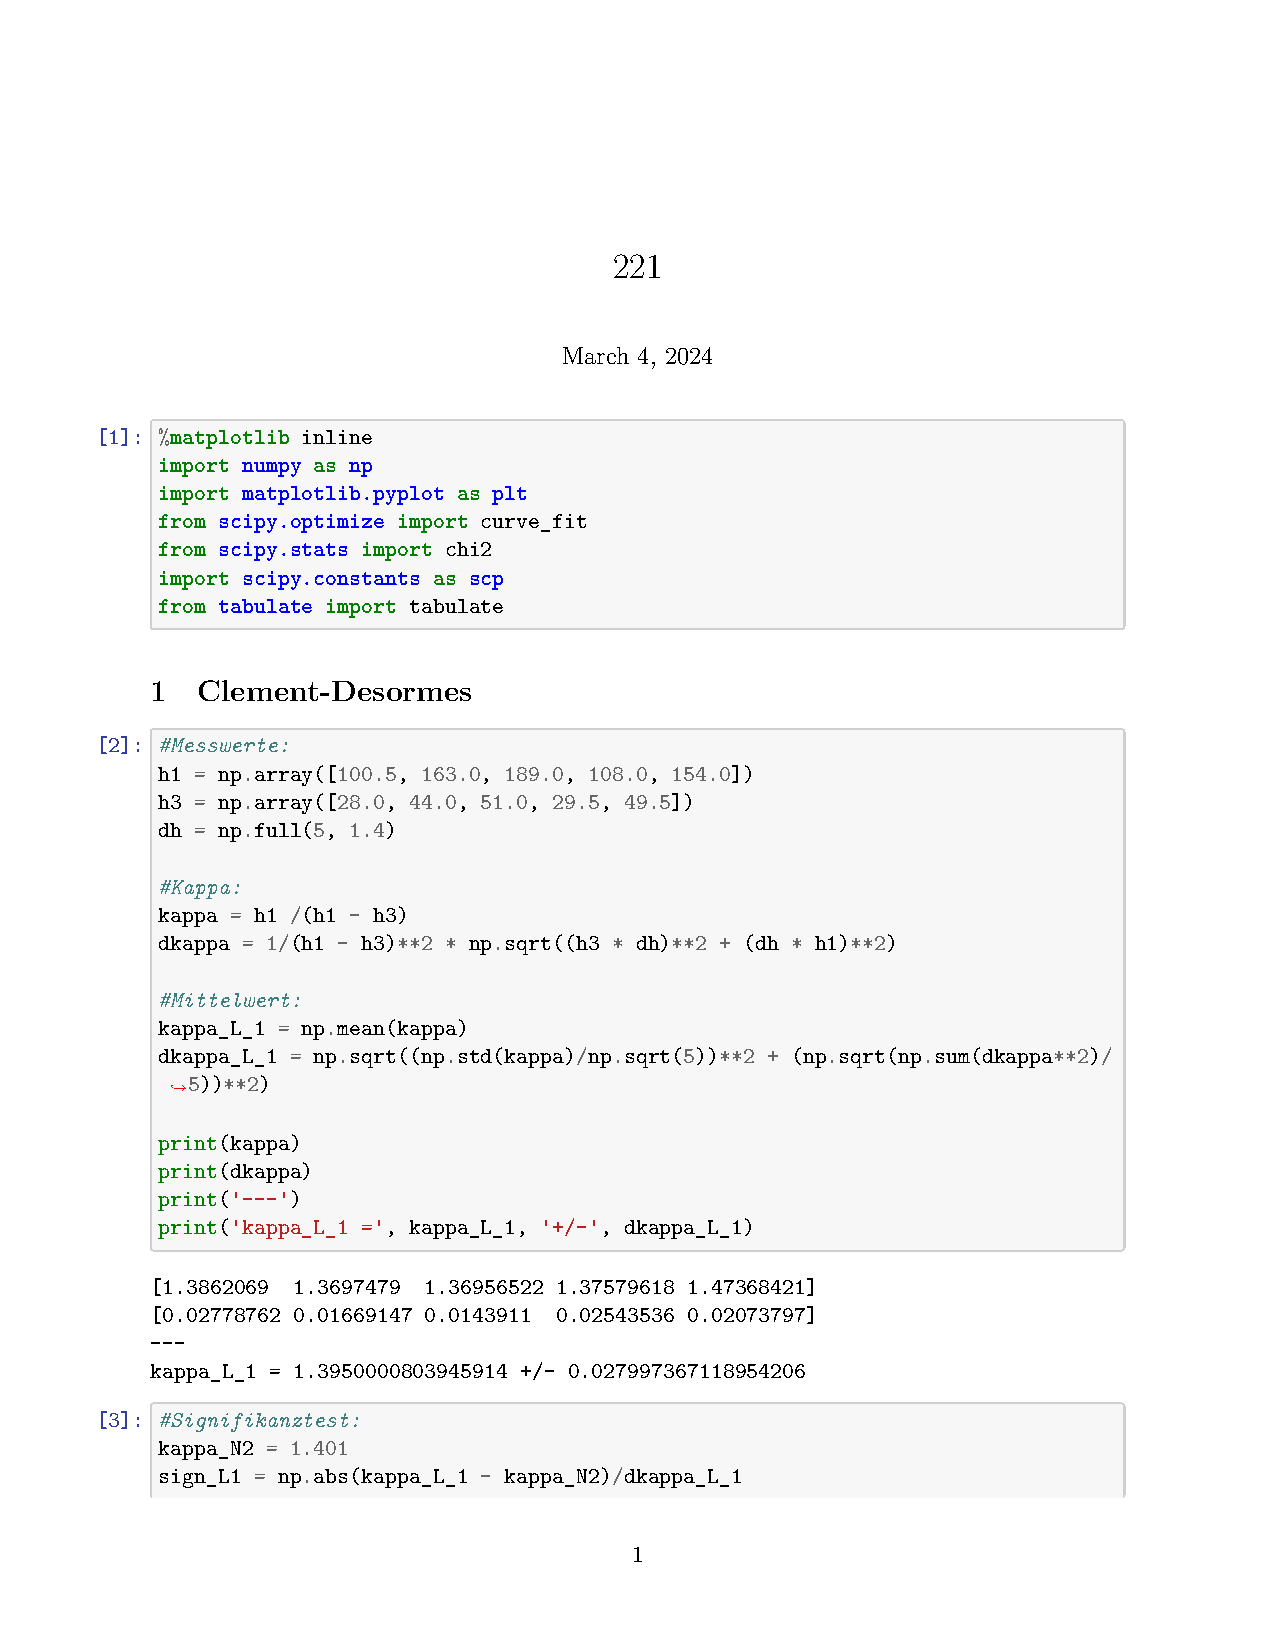
\includepdf[pages=-]{221.pdf}

\end{document}

